% \documentclass{book}

\documentclass[12pt]{article}
\usepackage[pdfborder={0 0 0.5 [3 2]}]{hyperref}%
\usepackage[left=1in,right=1in,top=1in,bottom=1in]{geometry}%
\usepackage[shortalphabetic]{amsrefs}%
\usepackage{amsmath}
\usepackage{enumerate}
\usepackage{enumitem}
\usepackage{amssymb}                
\usepackage{amsmath}                
\usepackage{amsfonts}
\usepackage{amsthm}
\usepackage{bbm}
\usepackage[table,xcdraw]{xcolor}
\usepackage{tikz}
\usepackage{float}
\usepackage{booktabs}
\usepackage{svg}
\usepackage{mathtools}
\usepackage{cool}
\usepackage{url}
\usepackage{graphicx,epsfig}
\usepackage{makecell}
\usepackage{array}

\def\noi{\noindent}
\def\T{{\mathbb T}}
\def\R{{\mathbb R}}
\def\N{{\mathbb N}}
\def\C{{\mathbb C}}
\def\Z{{\mathbb Z}}
\def\P{{\mathbb P}}
\def\E{{\mathbb E}}
\def\Q{\mathbb{Q}}
\def\ind{{\mathbb I}}

\graphicspath{ {images/} }

\begin{document}

\section{Introduction}

\section{Numerics}

\subsection{Parameter Continuation}

\subsection{Double Pulse Construction}

\begin{figure}[H]
	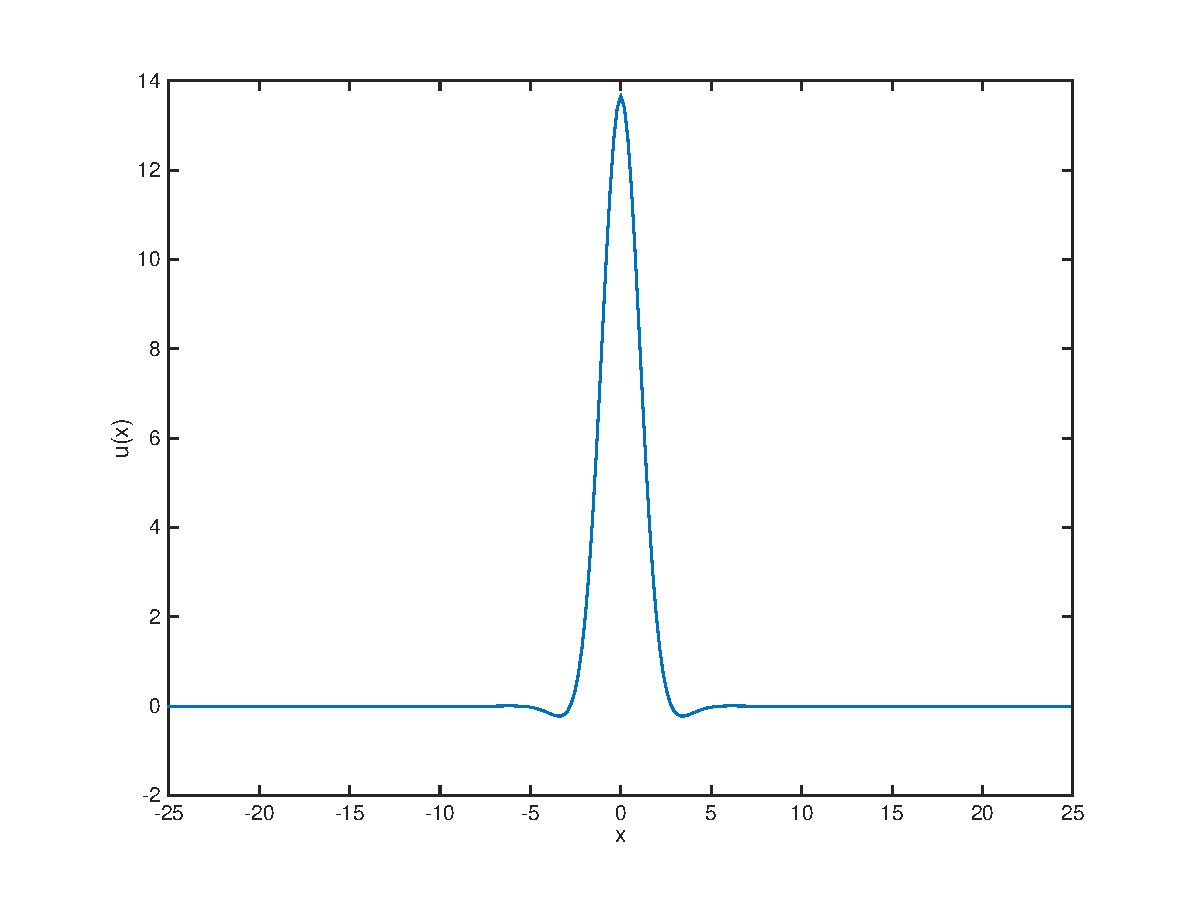
\includegraphics[width=8.5cm]{four10primary.eps}
	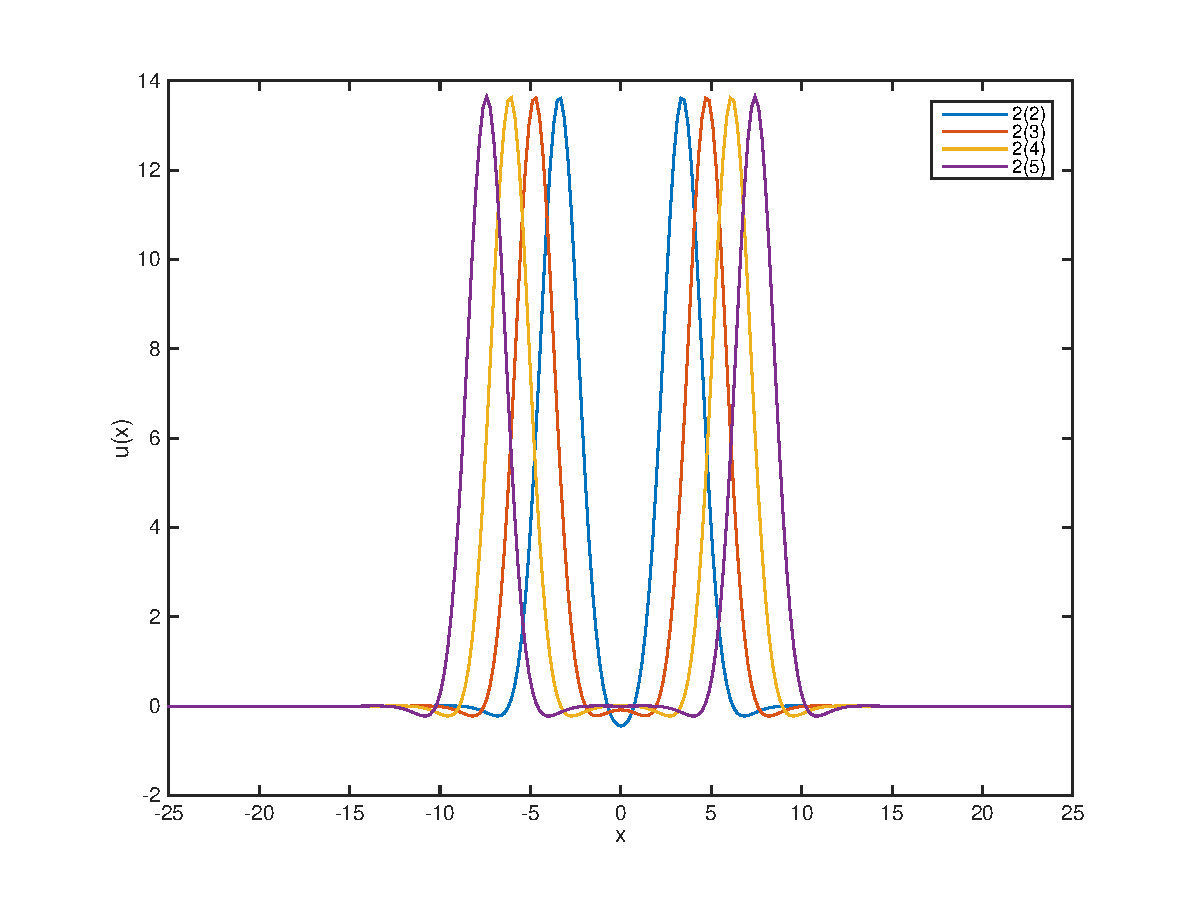
\includegraphics[width=8.5cm]{four10double.eps}
	\caption{Primary pulse and double pulses 2(2), 2(3), 2(4), and 2(5). Fourier spectral methods, $N = 256$, wave speed $c = 10$.}
\end{figure}

\begin{figure}[H]
	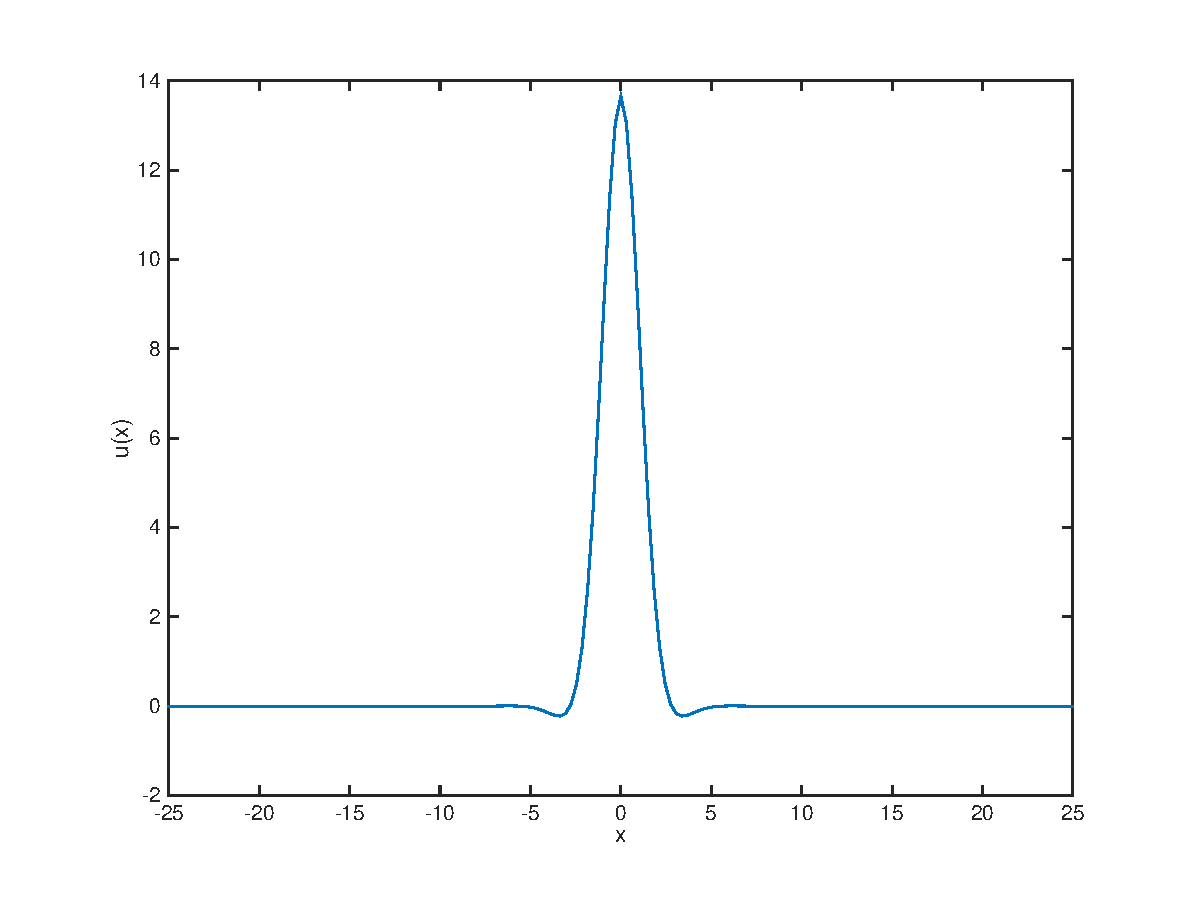
\includegraphics[width=8.5cm]{cheb10primary.eps}
	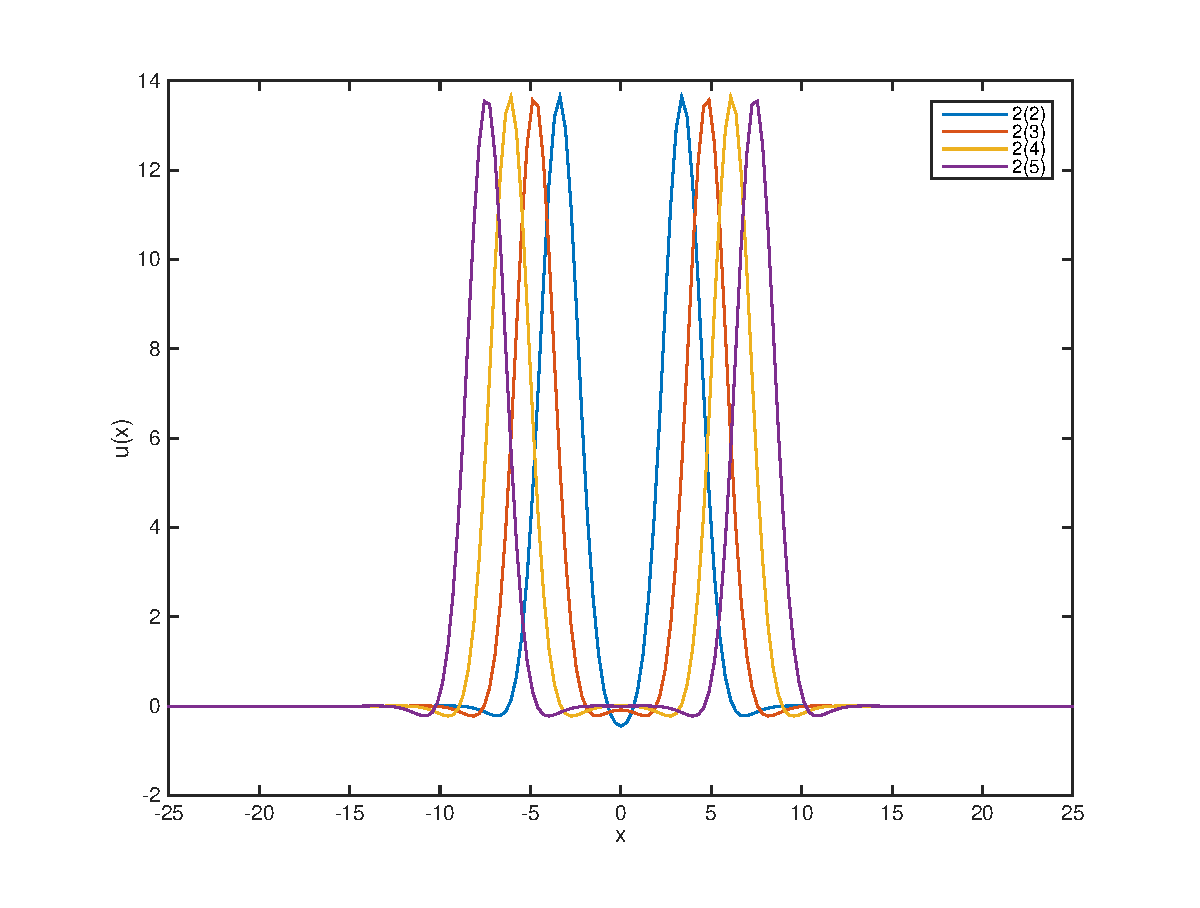
\includegraphics[width=8.5cm]{cheb10double}
		\caption{Primary pulse and double pulses 2(2), 2(3), 2(4), and 2(5). Chebyshev spectral methods, $N = 257$, wave speed $c = 10$.}
\end{figure}

\subsection{Eigenvalues}

\begin{figure}[H]
\begin{tabular}{l|lll}
 Double Pulse   & $c = 10$            & $c=7.5$                         & $c=5$        \\ \hline
  2(2) &     $\pm 0.4352$             & $\pm 0.2730$                    & $\pm 0.1363$ \\ 
  2(3) &     2.0829e-11 $\pm 0.0691i$ & -2.7698e-11 $\pm 0.0413i$       & 2.6806e-11 $\pm 0.0190i$\\ 
  2(4) &     $\pm 0.0109$             & $\pm 0.0062$                    & \\ 
  2(5) &    -8.5834e-13 $\pm 0.0020i$ & 6.8791e-12 $\pm$ 8.8812e-04$i$  & \\
\end{tabular}
\caption{Eigenvalues for linearization about double pulses 2(2), 2(3), 2(4), and 2(5) for wave speeds $c = 10, 7.5, 5$. Fourier spectral methods, $N = 256$}
\end{figure}

\begin{figure}[H]
\begin{tabular}{l|lll}
 Double Pulse   & $c = 10$            & $c=7.5$                        & $c=5$        \\ \hline
  2(2) &     $\pm 0.4352$             & $\pm 0.2730$                   & $\pm 0.1363$ \\ 
  2(3) &     3.5702e-08 $\pm 0.0691i$ & 1.2186e-08 $\pm 0.0413i$       & 2.0229e-09 $\pm 0.0190i$\\ 
  2(4) &     $\pm 0.0109$             & $\pm 0.0064$                   & \\ 
  2(5) &    -2.4222e-12 $\pm 0.0020i$ & 8.0169e-13 $\pm$ 9.4458e-04$i$ & \\
\end{tabular}
\caption{Eigenvalues for linearization about double pulses 2(2), 2(3), 2(4), and 2(5) for wave speeds $c = 10, 7.5, 5$. Chebyshev spectral methods, $N = 257$}
\end{figure}

\subsection{Time stepping}

\section{References}

\end{document}